\documentclass[10pt,landscape]{article}
\usepackage{multicol}
\usepackage{calc}
\usepackage{ifthen,graphicx}
\usepackage[landscape]{geometry}
\usepackage{sidecap}
\usepackage{nonfloat}
\usepackage{lipsum}
\newenvironment{Figure}
  {\par\medskip\noindent\minipage{\linewidth}}
  {\endminipage\par\medskip}
\newcommand\myfigure[1]{%
\medskip\noindent\begin{minipage}{\columnwidth}
\centering%
#1%
%figure,caption, and label go here
\end{minipage}\medskip}
% To make this come out properly in landscape mode, do one of the following
% 1.
%  pdflatex latexsheet.tex
%
% 2.
%  latex latexsheet.tex
%  dvips -P pdf  -t landscape latexsheet.dvi
%  ps2pdf latexsheet.ps


% If you're reading this, be prepared for confusion.  Making this was
% a learning experience for me, and it shows.  Much of the placement
% was hacked in; if you make it better, let me know...


% 2008-04
% Changed page margin code to use the geometry package. Also added code for
% conditional page margins, depending on paper size. Thanks to Uwe Ziegenhagen
% for the suggestions.

% 2006-08
% Made changes based on suggestions from Gene Cooperman. <gene at ccs.neu.edu>


% To Do:
% \listoffigures \listoftables
% \setcounter{secnumdepth}{0}


% This sets page margins to .5 inch if using letter paper, and to 1cm
% if using A4 paper. (This probably isn't strictly necessary.)
% If using another size paper, use default 1cm margins.
\ifthenelse{\lengthtest { \paperwidth = 11in}}
	{ \geometry{top=.5in,left=.5in,right=.5in,bottom=.5in} }
	{\ifthenelse{ \lengthtest{ \paperwidth = 297mm}}
		{\geometry{top=1cm,left=1cm,right=1cm,bottom=1cm} }
		{\geometry{top=1cm,left=1cm,right=1cm,bottom=1cm} }
	}

% Turn off header and footer
\pagestyle{empty}
 

% Redefine section commands to use less space
\makeatletter
\renewcommand{\section}{\@startsection{section}{1}{0mm}%
                                {-1ex plus -.5ex minus -.2ex}%
                                {0.5ex plus .2ex}%x
                                {\normalfont\large\bfseries}}
\renewcommand{\subsection}{\@startsection{subsection}{2}{0mm}%
                                {-1explus -.5ex minus -.2ex}%
                                {0.5ex plus .2ex}%
                                {\normalfont\normalsize\bfseries}}
\renewcommand{\subsubsection}{\@startsection{subsubsection}{3}{0mm}%
                                {-1ex plus -.5ex minus -.2ex}%
                                {1ex plus .2ex}%
                                {\normalfont\small\bfseries}}
\makeatother

% Define BibTeX command
\def\BibTeX{{\rm B\kern-.05em{\sc i\kern-.025em b}\kern-.08em
    T\kern-.1667em\lower.7ex\hbox{E}\kern-.125emX}}

% Don't print section numbers
\setcounter{secnumdepth}{0}


\setlength{\parindent}{0pt}
\setlength{\parskip}{0pt plus 0.5ex}


% -----------------------------------------------------------------------

\begin{document}

\raggedright
\footnotesize
\begin{multicols}{3}


% multicol parameters
% These lengths are set only within the two main columns
%\setlength{\columnseprule}{0.25pt}
\setlength{\premulticols}{1pt}
\setlength{\postmulticols}{1pt}
\setlength{\multicolsep}{1pt}
\setlength{\columnsep}{2pt}

\begin{center}
     \Large{CS170 cribsheet midterm1} \\
\end{center}

\section{Order of Growth}
\subsection{Formal}
\newlength{\MyLen}
\settowidth{\MyLen}{\texttt{letterpaper}/\texttt{a4paper} \ }

UpperBound $O$ : LowerBound $\Omega$ : Constant $\Theta$
$\frac{a(n)}{b(n)}>0, a(n)\in \Omega(b(n))$
$\frac{a(n)}{b(n)}<c, a(n)\in O(b(n))$
$\frac{a(n)}{b(n)}=c, a(n)\in \Theta(b(n))$

\subsection{Tricks}
\settowidth{\MyLen}{\texttt{letterpaper}/\texttt{a4paper} \ }
$7^{\log(n)^2}=(2^{\log(7)})^{(\log(n))^2}=(2^{\log(n)})^{\log(7)\log(n)}\approx n^{\log(n)}$

$n! = 2^{n\log(n)}$ ::$36^5=6^{10}$ 

Solve the comparison by integration.
 
$(a+bi)*(c+di)\rightarrow r=ab,s=bd,t=(a+b)(c+d) = r-s+(t-r-s)i$

\subsection{add/multiply}

Karatsuba's $= \Theta(n^{\log_2{3}})$
\subsection{Prove}

Geom sum series: $g(n)=\frac{1-c^{n+1}}{1-c} = \frac{c^{n+1}-1}{c-1}$

Induction: $\gcd(F_{k+1},F_{k+1}) = \gcd(F_{k+1},F_{k+2}-F_{K+1}) = \gcd(F_{k+1},F_{k}) =1$

Numbers before prime $1/n$: in $O(n)$ time. Geom dist.$E[X]=\sum^{\infty}_{i=1}{i*P[X=i]}=\sum^{\infty}_{i=1}{i*(1-p)^{(i-1)}p}$ $p=probheads, i-1=tails throws$ 
$= p * dp/dt (\sum^{\infty}_{i=1}{-(1-p)^i})\rightarrow_{sums}=-1/p$ Integrate: $E[X]=p*(1/p^2)=1/p$ 

Binary Search: if $N$ is a square. Why only $\log n$ for power max? $N=q^k\rightarrow \log N=k\log \rightarrow k=\log N/\log q \leq \log N$ 

For any power: poweringoperation\{$\sum^{k}_{i=1}{in*n}=O(k^2n^2)$\} Repeat $\log n $ times to get $O(n^6)$

\subsection{Modular Arithmetic}
Quadratic residue busniess.
Fermat's theorem: $\forall 1\leq a < p: a^{p-1}\equiv1modp$ if p is prime.

Euler's Theorem: $m^{(p-1)(q-1)}\equiv 1 (mod pq)$
Multitudes: $2013^{2014}= 3^{2012+2}=(3^{503})^4*3^2=1*3^2=4 all mod 5$
$2012^{2013}=2^{2012+1}=(2^{503})^2*2^1=1*2=2 all mod 5$
$5^{170^{70}} mod 5$: take $170^{70}=4s+t$ form $170^{70}=(2*85)^{(2*35)}=(4*85^2)^{35}=0mod4$ 

Worst RSA: We know N,e,d: $k=(ed-1)/(p-1)(q-1)$, limit k$\in 1,2$ by $e=3,d<(p-1)(q-1)$ Solve two eq system for p and q modulating k, use $N=pq$.

Randomize recoverable RSA w/ $(M^e*k^e)^d mod N=MkmodN$ then multiply by $k^{-1}$

Primality testing: Doesn't catch Carmichaels. you did this for euler project already
\section{Divide and Conquer}
Master's Theorem: $T(n)=aT({n/b})+O(n^d),a>0,b>1,d\geq 0$

$O(n^d) \rightarrow d>\log_b{a}$ ::
$O(n^d\log n) \rightarrow d=\log_b{a}$ ::
$O(n^{\log_b{a}}) \rightarrow d<\log_b{a}$

Majority Element: If there is a majority element then it will be a majority element of $A_1$ or $A_2,, O(n\log n)$. Or you could use the pairing-discard approach $T(n)=T(n/2)+O(n)=O(n)$

For finding kth smallest element in array, $O(n) average, O(n^2) worst$
\begin{Figure}
 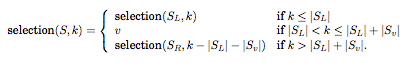
\includegraphics[scale=0.5]{selection}
\end{Figure}
% {%
% \setlength{\fboxsep}{0pt}%
% \setlength{\fboxrule}{0pt}%
% \fbox{\includegraphics[scale=0.25]{"unit_circle"}}%
% }%
\begin{Figure}
 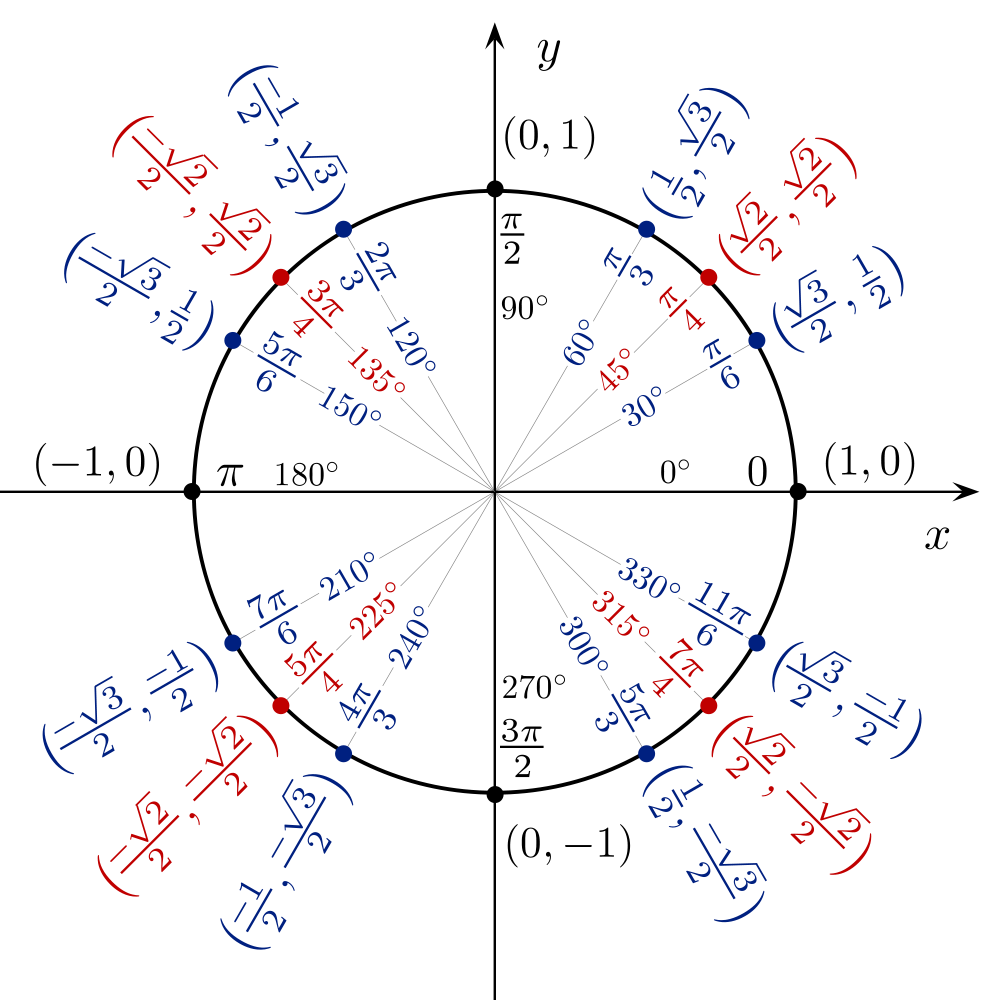
\includegraphics[scale=0.2]{unit_circle_2}
\end{Figure}
%
% \myfigure{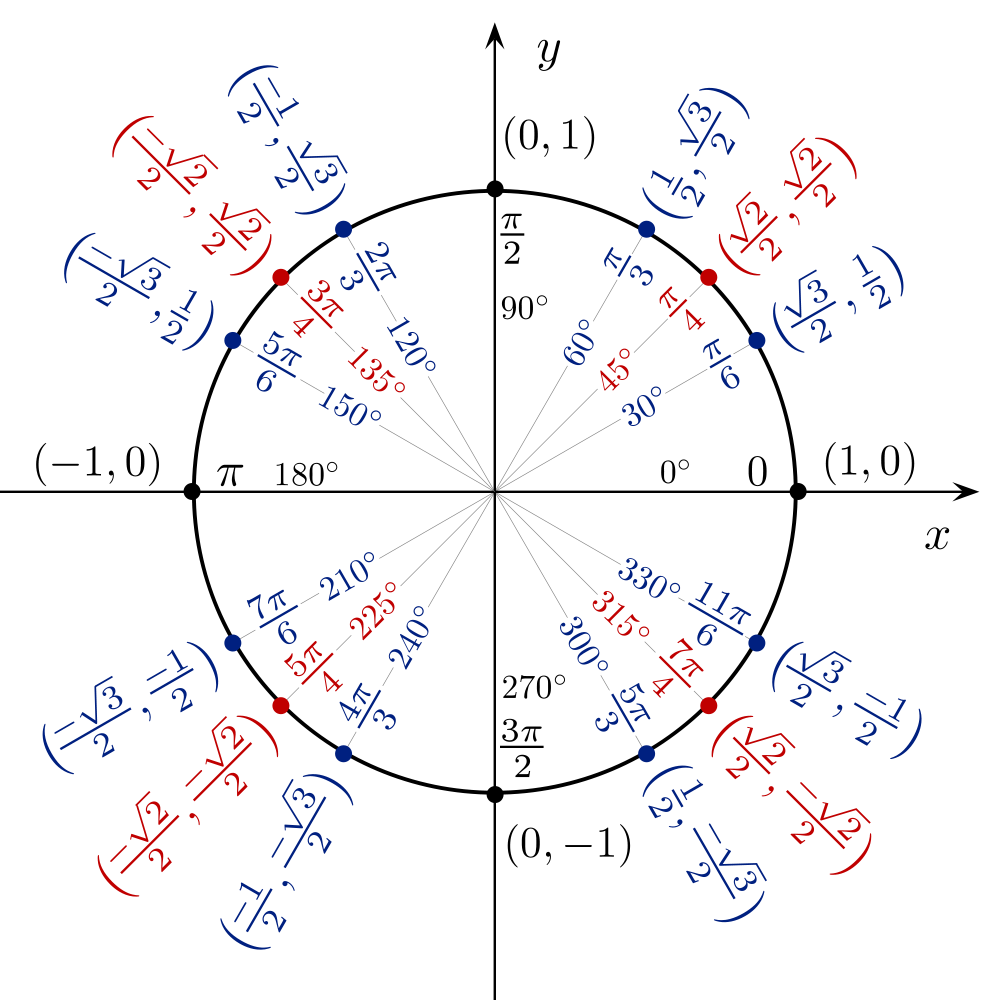
\includegraphics[width=.5\columnwidth]{unit_circle_2}%
% \figcaption{\emph{I am a figure caption!}}}
%

% \includegraphics[scale=0.25]{"unit_circle"}
Complex number practice: $\omega = e^{2\pi i/8},n=8,=\sqrt{2}/2 + i\sqrt{2}/2$

$\omega^7 = e^{2\pi i (7/8)}=\sqrt{2}/2 - i\sqrt{2}/2=\omega^-1,\omega^7 + \omega = \sqrt{2}$
$p(x)=x^2+1, p(\omega)=1+i,p(\omega^2)=0,p(\omega^3)=1-i$


Missing integer: Array A of numbers [0,N]. Split into N/2 and count the bits in least significant position. You know how may 1-bits to expect. If that number is spot on, missing=0, otherwise missing=1. For each of these splits and counts we downsize by N/2 $\rightarrow T(n)=T(n/2)+O(n)=O(n)$, all without bit complexity

Pareto points: Sort $O(n\log n)$ and then do  linear scan in reverse order $O(n)$



FFT: $A(x)=1+2x-x^2+3x^3$ $(x_1,x_2,x_3,x_4)=(\omega^0,\omega^1,\omega^2,\omega^3)=(1,i,-1,-i)::\omega=e^{2\pi i/n}$ In general find the nearest power of two as \emph{n}

Split into $A(x)=A_e(x)+xA_o(x)::A_e(x)=1-x,A_o(x)=2+3x$
$A_e(\omega^{2j})+\omega^iA_o(\omega^{2j})$

DFT Matrix entry: $(m,n)=\omega^{m*n}=e^{(2\pi i/n)*mn}$
Inverse DFT AMmtrix entry:  $(m,n)=(1/n)*\omega^{-m*n}=e^{-(2\pi i/n)*mn}$

\begin{Figure}
 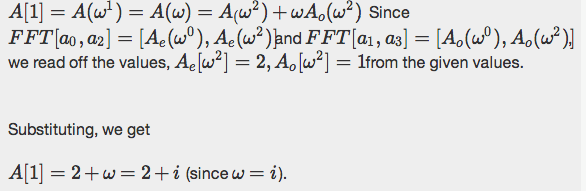
\includegraphics[scale=0.35]{FFT_example}
\end{Figure}

\begin{Figure}
 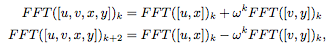
\includegraphics[scale=0.7]{FFT}
\end{Figure}


\section{Graphs}
\subsection{Facts}
Undirec graph w/ n verts and n edges has cycle by induction.

Stongly connected: path between any two points
:: TREE EDGES $<=>$ CROSS EDGES depending on DFS

Dijkstra's: Put all edges on a list and mark distance $\infty$, $O(|V|)$ time.

\begin{Figure}
 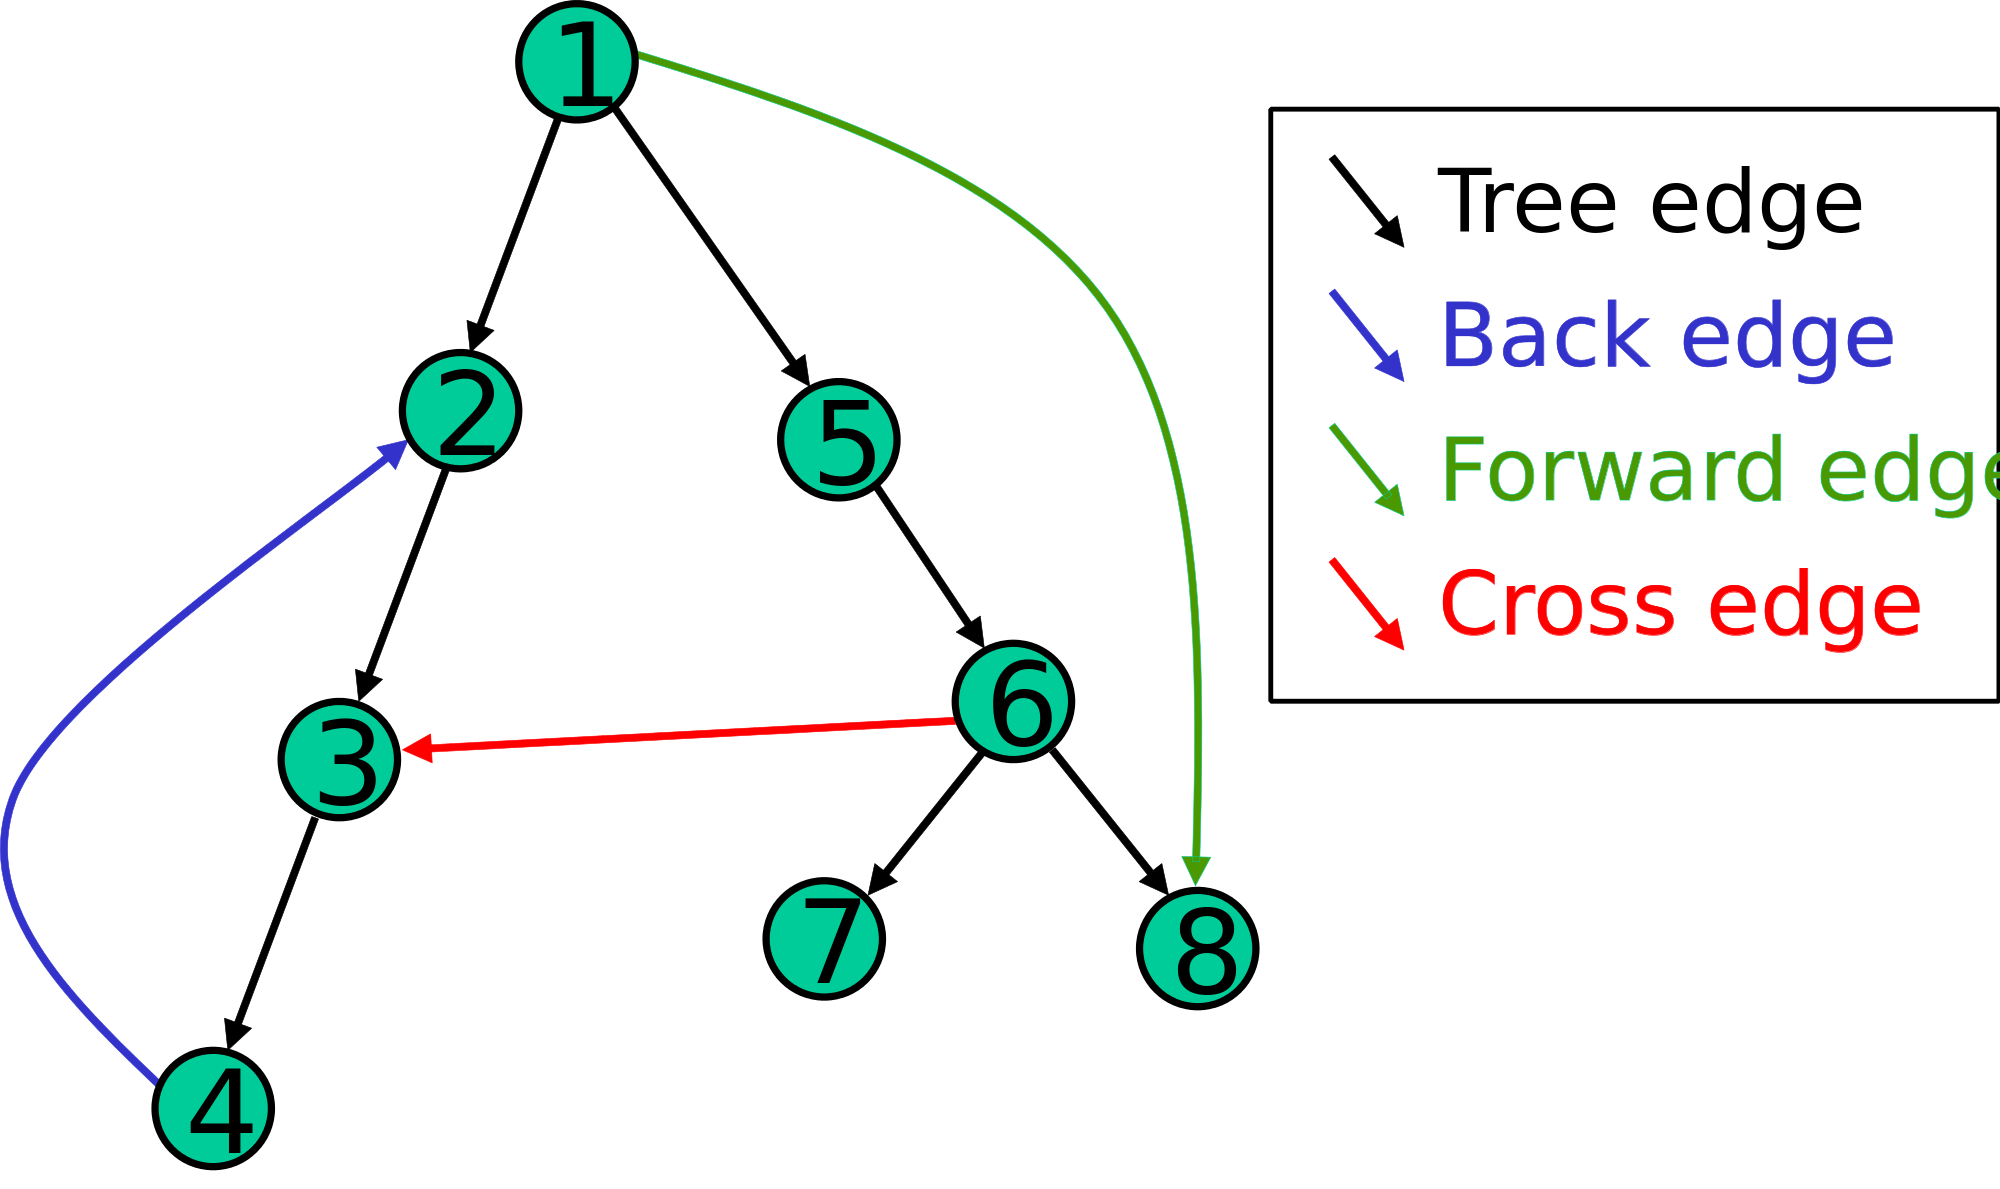
\includegraphics[scale=0.08]{tree_edges}
\end{Figure}

\begin{Figure}
    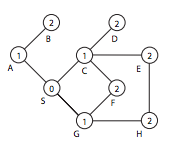
\includegraphics[scale=0.7]{BFS}
\end{Figure}

\begin{Figure}
 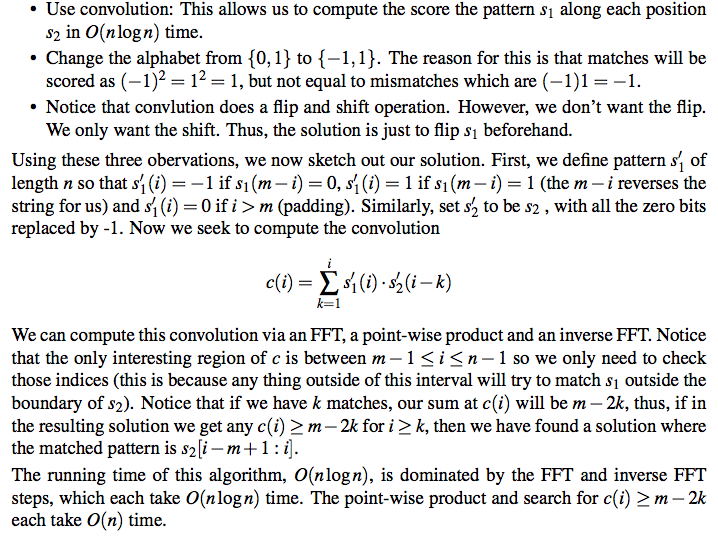
\includegraphics[scale=0.3]{convolution}
\end{Figure}
\rule{0.3\linewidth}{0.25pt}
\scriptsize



2013 Zack Field


\end{multicols}
\end{document}